\label{sec:sym_verschl}

Die symmetrische Verschlüsselung folgt dem Konzept, das sowohl für die Ver- als auch die Entschlüsselung jeweils die gleichen Schlüssel verwendet werden. \\
Abbildung~\ref{fig:sym_verschl} zeigt eine schematische Darstellung.

\begin{figure}[h!]
	\centering
	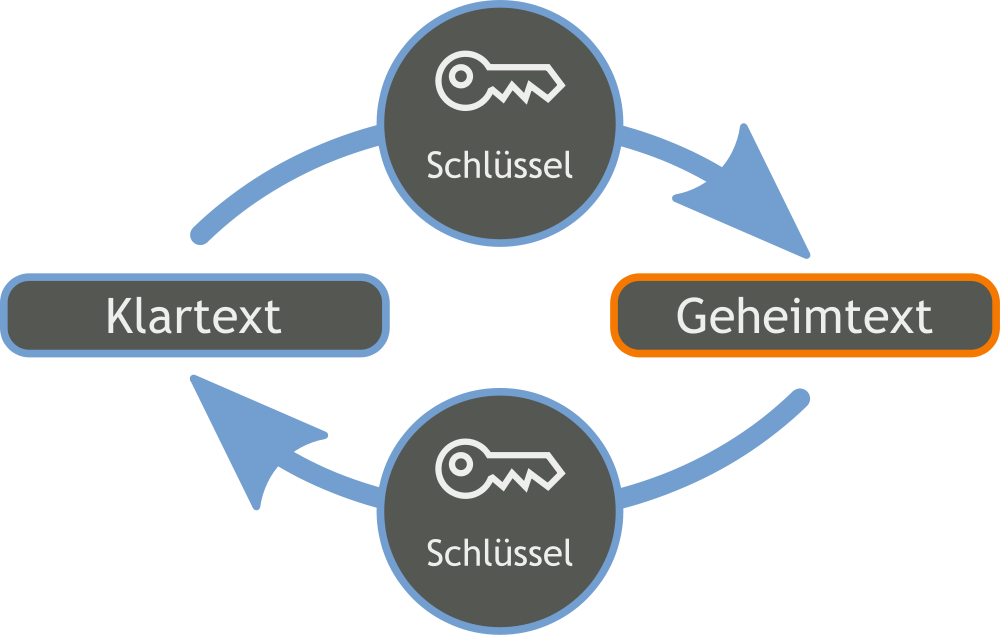
\includegraphics[scale=0.22]{img/SymKrypto.png}
	\caption{Symmetrische Verschlüsselung mit identischen Schlüsseln \\
	Bananenfalter (Public Domain) \\ \url{https://commons.wikimedia.org/wiki/File:Orange_blue_symmetric_cryptography_de.svg}
	}
	\label{fig:sym_verschl}
\end{figure}

Es gibt eine Reihe an unterschiedlichsten Algorithmen und Verfahren für symmetrische Verschlüsselung, allerdings hat sich mit \texttt{AES} ein Verfahren als de-facto Standard für verschiedenste Anwendungsbereiche etabliert.

\texttt{AES} ist hierbei eine Abkürzung für \texttt{Advanced Encryption Standard} und wird meist synonym für den \texttt{Rijndael}-Algorithmus verwendet. Dieses Verfahren ist heute so verbreitet, dass es beispielsweise in modernen Prozessoren direkt als Maschinenbefehl zur Verfügung steht \cite{crypto:aes_intel}. 
\\

Bei Ransomware ist es während der Phase, in der die eigentliche Dateiverschlüsselung durchgeführt wird, wichtig, nicht vom Opfer erkannt zu werden. Allerdings würde es wahrscheinlich auf unkundigen Nutzern auffallen, wenn der Computer auf Eingaben nur noch verzögert reagiert, wie es typischerweise geschieht, wenn die \texttt{CPU} im Hintergrund mit rechenintensiven Aufgaben, zu denen auch Verschlüsselungsoperationen gehören, ausgelastet ist.

Mittels der Hardwarebeschleunigung wird zwar die \texttt{CPU}-Belastung reduziert, dennoch ist oftmals eine Verlangsamung des Computers festzustellen, vor allem bedingt durch die großen Datenmengen die vom den angeschlossenen Speichergeräten gelesen und verschlüsselt geschrieben werden müssen.

Sowohl für den Entwickler als auch den Betreiber der Ransomware ist es hier vorteilhaft eine gewisse Lastbegrenzung, sowohl für Speicher als auch \texttt{CPU}, einzubauen bzw. zu verwenden.
\\

Der größte Nachteil beim Einsatz von symmetrischer Verschlüsselung ist allerdings die Eigenschaft, dass sowohl für die Ver- als auch für die Entschlüsselung der gleiche Schlüssel verwendet wird. Prinzipbedingt muss der Schlüssel während der Verschlüsselung einer Datei im \texttt{RAM} gehalten werden und kann somit von anderen Programmen ausgelesen werden.

Wird ein Schlüssel für mehrere oder auch alle Dateien verwendet, so stellt das Auslesen des verwendeten Schlüssels aus dem \texttt{RAM} ein gute Möglichkeit dar, ohne Zahlung die verschlüsselten Dateien wird zu decodieren. 

Diese prinzipielle Schwäche einer symmetrischen Verschlüsselung lässt sich durch die Verwendung asymmetrischer Verschlüsselung umgehen.

\subsection{Asymmetrische Verschlüsselung}
\label{sec:asym_verschl}

\begin{figure}[h!]
	\centering
	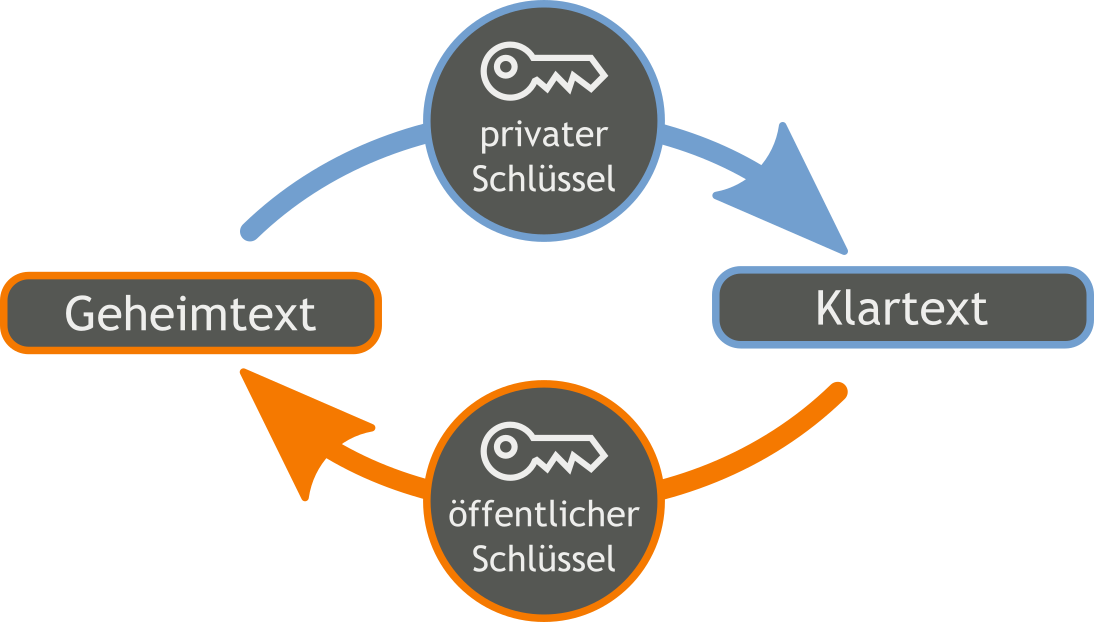
\includegraphics[scale=0.25]{img/AsymKrypto.png}
	\caption{Asymmetrische Verschlüsselung \\
	Bananenfalter (Public Domain) \\ \url{https://commons.wikimedia.org/wiki/File:Orange_blue_symmetric_cryptography_de.svg}}
	\label{fig:asym_verschl}
\end{figure}

Asymmetrische Verschlüsselung basiert auf zwei Schlüsseln, einem öffentlichen und einem privaten. Diese Schlüssel gehören mathematisch zusammen und werden für unterschiedliche Zwecke verwendet.

Soll ein Klartext verschlüsselt werden, so wird hierfür der öffentliche Schlüssel des Empfängers verwendet. Die Entschlüsselung muss dann mit dem zugehörigen privaten Schlüssel erfolgen, eine Entschlüsselung mit dem öffentlichen Schlüssel ist nicht mehr möglich.

Es existieren mehrere genaue Verfahren für asymmetrische Verschlüsselung. Die Bekanntesten sind hier das \texttt{RSA}-Verfahren und das \texttt{Elgamal}-Verfahren.\\
Beide Verfahren unterscheiden sich zwar mathematisch stark voneinander, da \texttt{RSA} auf dem Problem der Primfaktorzerlegung basiert, während sich \texttt{Elgamal} auf die Schwierigkeit des diskreten Logarithmus stützt. \\
Hinsichtlich ihrer Verwendung und Sicherheit im Umfeld von Ransomware sind sich beide Verfahren ebenbürtig, weshalb im weiteren nur das \texttt{RSA}-Verfahren behandelt wird.
\\

Auf Grund der Komplexität der Berechnungen ist \texttt{RSA} im Vergleich zu \texttt{AES} langsam \cite{crypto:aes_rsa_benchmark}. Deshalb wird es nur für verhältnismäßig kurze Klartexte eingesetzt (< 1 KB), auch da die maximale Länge des Klartexts von der Länge des verwendeten Schlüssels abhängt. %TODO: Nachweis
\\

Der große Vorteil von asymmetrischer Verschlüsselung liegt im sicheren Schlüsselaustausch, der nicht auf einen bereits gesicherten Kanal angewiesen ist, sondern auch über ein unsicheres Medium, beispielsweise über das Internet erfolgen kann, ohne dass es für einen Angreifer möglich ist die beteiligten Schlüssel zu belauschen oder zu berechnen. %TODO: MitM




\subsection{Hybride Verschlüsselung}
\label{sec:hybride_verschl}

Hybride Verschlüsselung kombiniert alle Vorteile von symmetrischer Verschlüsselung (Geschwindigkeit, Einfachheit) mit allen Vorteilen von asymmetrischer Verschlüsselung (Schlüsseltausch, Sicherheit).
Hierfür werden zufällige Schlüssel erzeugt, meist lange Zufallszahlen, die für die symmetrische Verschlüsselung verwendet werden. Diese Schlüssel werden Sitzungsschlüssel genannt und werden in der Regel nur einmalig verwendet (ein sog. One-Time-Pad). Nach der Verwendung werden die Sitzungsschlüssel asymmetrisch verschlüsselt und mit den codierten Daten zusammen übertragen.

Auf diese Weise lassen sich auch große Mengen an Daten effizient mittels asymmetrischer Kryptographie übertragen.
